\documentclass[table]{beamer}
%[]中可以使用draft、handout、screen、transparency、trancompress、compress等参数

%指定beamer的模式与主题
\mode<presentation>
{
  \usetheme{Madrid}
%\usetheme{Boadilla}
%\usecolortheme{default}
%\usecolortheme{orchid}
%\usecolortheme{whale}
%\usefonttheme{professionalfonts}
}

%\usetheme{Madrid}
%这里还可以选择别的主题:Bergen, Boadilla, Madrid, AnnArbor, CambridgeUS, Pittsburgh, Rochester, Warsaw, ...
%有导航栏的Antibes, JuanLesPins, Montpellier, ...
%有内容的Berkeley, PaloAlto, Goettingen, Marburg, Hannover, ...
%有最小导航栏的Berlin, Ilmenau, Dresden, Darmstadt, Frankfurt, Singapore, Szeged, ...
%有章和节表单的Copenhagen, Luebeck, Malmoe, Warsaw, ...

%\usecolortheme{default}
%设置内部颜色主题(这些主题一般改变block里的颜色);这个主题一般选择动物来命名
%这里还可以选择别的颜色主题,如默认的和有特别目的的颜色主题default,structure,sidebartab,全颜色主题albatross,beetle,crane,dove,fly,seagull,wolverine,beaver

%\usecolortheme{orchid}
%设置外部颜色主题(这些主题一般改变title里的颜色);这个主题一般选择植物来命名
%这里还可以选择别的颜色主题,如默认的和有特别目的的颜色主题lily,orchid,rose

%\usecolortheme{whale}
%设置字体主题;这个主题一般选择海洋动物来命名
%这里还可以选择别的颜色主题,如默认的和有特别目的的颜色主题whale,seahorse,dolphin

%\usefonttheme{professionalfonts}
%类似的还可以定义structurebold,structuresmallcapsserif,professionalfonts

% 控制 beamer 的风格,可以根据自己的爱好修改
%\usepackage{beamerthemesplit} %使用 split 风格
%\usepackage{beamerthemeshadow} %使用 shadow 风格
%\usepackage[width=2cm,dark,tab]{beamerthemesidebar}

%插入音标
%\usepackage{tipa}
%\AtBeginDocument{
  %\renewcommand\textipa{\fontencoding{T3}\selectfont}
%}
%\AtBeginDocument{
  %\renewcommand\textipa[2][r]{{\fontfamily{cm#1}\tipaencoding #2}}
%}
%\renewenvironment{IPA}[1][r]
 %{\fontfamily{cm#1}\tipaencoding}
 %{}

% 设定英文字体
%\usepackage{fontspec}
% Fix bugs for fontspec in TeXLive2015
\ifdefined\suppressfontnotfounderror
  \expandafter\let\csname xetex_suppressfontnotfounderror:D\endcsname
    \suppressfontnotfounderror
\else
  \expandafter\let\csname xetex_suppressfontnotfounderror:D\endcsname
    \luatexsuppressfontnotfounderror
\fi
\usepackage[no-math]{fontspec}
\setmainfont{Times New Roman}
\setsansfont{Arial}
\setmonofont{Courier New}

% 设定中文字体
\usepackage[BoldFont,SlantFont,CJKchecksingle,CJKnumber]{xeCJK}
%\setCJKmainfont[BoldFont={Adobe Heiti Std},ItalicFont={Adobe Kaiti Std}]{Adobe Song Std}
\setCJKmainfont[BoldFont={Adobe Heiti Std},ItalicFont={Adobe Kaiti Std}]{WenQuanYi Micro Hei}
\setCJKsansfont{Adobe Heiti Std}
\setCJKmonofont{Adobe Fangsong Std}
\punctstyle{hangmobanjiao}

\defaultfontfeatures{Mapping=tex-text}
\usepackage{xunicode}
\usepackage{xltxtra}

\XeTeXlinebreaklocale "zh"
\XeTeXlinebreakskip = 0pt plus 1pt minus 0.1pt

\usepackage{setspace}
\usepackage{colortbl,xcolor}
\usepackage{hyperref}
%\hypersetup{xetex,bookmarksnumbered=true,bookmarksopen=true,pdfborder=1,breaklinks,colorlinks,linkcolor=blue,filecolor=black,urlcolor=cyan,citecolor=green}
\hypersetup{xetex,bookmarksnumbered=true,bookmarksopen=true,pdfborder=1,breaklinks,colorlinks,linkcolor=cyan,filecolor=black,urlcolor=blue,citecolor=green}

% 插入图片
\usepackage{graphicx}
\graphicspath{{figures/}}
% 图文混排
%\usepackage{picins}
\usepackage{floatflt}

% 可能用到的包
\usepackage{amsmath,amssymb}
%插入多媒体
%\usepackage{media9}
%\usepackage{movie15}
\usepackage{multimedia}
\usepackage{multicol}
\usepackage{multirow}

% 定义一些自选的模板,包括背景、图标、导航条和页脚等,修改要慎重
% 设置背景渐变由10%的红变成10%的结构颜色
%\beamertemplateshadingbackground{red!10}{structure!10}
%\beamertemplatesolidbackgroundcolor{white!90!blue}
% 使所有隐藏的文本完全透明、动态,而且动态的范围很小
\beamertemplatetransparentcovereddynamic
% 使itemize环境中变成小球,这是一种视觉效果
\beamertemplateballitem
% 为所有已编号的部分设置一个章节目录,并且编号显示成小球
\beamertemplatenumberedballsectiontoc
% 将每一页的要素的要素名设成加粗字体
\beamertemplateboldpartpage

% item逐步显示时,使已经出现的item、正在显示的item、将要出现的item呈现不同颜色
\def\hilite<#1>{
 \temporal<#1>{\color{gray}}{\color{blue}}
    {\color{blue!25}}
}

\renewcommand{\today}{\number\year 年 \number\month 月 \number\day 日}

%五角星
\usepackage{MnSymbol}

%去除图表标题中的figure等
\usepackage{caption}
\captionsetup{labelformat=empty,labelsep=none}

\usepackage{tabu}
\usepackage{multirow}
%表格自动换行
\usepackage{tabularx} 

% 千分号
%\usepackage{textcomp}

%罗马数字
\makeatletter
\newcommand{\rmnum}[1]{\romannumeral #1}
\newcommand{\Rmnum}[1]{\expandafter\@slowromancap\romannumeral #1@}
\makeatother

%分栏
\usepackage{multicol}

%\usepackage{enumitem}
%\usepackage{enumerate}

%键盘
\usepackage{keystroke}

%心形
%\usepackage{fdsymbol}

%插入源代码
\usepackage{listings}
\lstset{
  language=perl,                  % 程序语言名称:TeX, Perl, R, sh, bash, Awk
  basicstyle=\normalsize\tt,      %\tt指monospace字体族,程序源代码使用此族字体表示更加美观
  numbers=left,                   % 行号位置(左侧)
  numberstyle=\small,             % 行号字体的字号
  stepnumber=1,                   % 行号的显示步长
  numbersep=5pt,                  % 行号与代码间距
  backgroundcolor=\color{white},  % 背景色;需要 \usepackage{color}
  showspaces=false,               % 不显示空格
  showstringspaces=false,         % 不显示代码字符串中的空格标记
  showtabs=false,                 % 不显示 TAB
  tabsize=4, 
  frame=shadowbox,                % 把代码用带有阴影的框圈起来
  captionpos=b,                   % 标题位置
  breaklines=true,                % 对过长的代码自动断行
  breakatwhitespace=false,        % 断行只在空格处
  extendedchars=false,            % 解决代码跨页时,章节标题,页眉等汉字不显示的问题
  %escapeinside={\%*}{*},         % 跳脱字符,添加注释,暂时离开 listings 
  %escapeinside=``,
  commentstyle=\color{red!50!green!50!blue!50}\tt,  %浅灰色的注释
  rulesepcolor=\color{red!20!green!20!blue!20},     %代码块边框为淡青色
  keywordstyle=\color{blue!70}\bfseries\tt,         %代码关键字的颜色为蓝色,粗体
  identifierstyle=\tt,
  stringstyle=\tt,                % 代码字符串的特殊格式
  keepspaces=true,
  breakindent=1em,
  %breakindent=22pt,
  %breakindent=4em,
  breakautoindent=true,
  flexiblecolumns=true,
  aboveskip=1em,                  %代码块边框
  xleftmargin=2em,
  xrightmargin=2em
}

%\setbeamercolor{alerted text}{fg=magenta}
\setbeamercolor{bgcolor}{fg=yellow,bg=cyan}
%\setbeamercolor{itemize/enumerate body}{fg=green}

\begin{document}

%\includeonlyframes{current}

\logo{
\includegraphics[height=0.08\textwidth]{qr.png}}

% 在每个Section前都会加入的Frame
\AtBeginSection[]
{
  \begin{frame}<beamer>
    %\frametitle{Outline}
    \frametitle{教学提纲}
    \setcounter{tocdepth}{3}
    \begin{multicols}{2}
      \tableofcontents[currentsection,currentsubsection]
      %\tableofcontents[currentsection]
    \end{multicols}
  \end{frame}
}
% 在每个Subsection前都会加入的Frame
\AtBeginSubsection[]
{
  \begin{frame}<beamer>
%%\begin{frame}<handout:0>
%% handout:0 表示只在手稿中出现
    \frametitle{教学提纲}
    \setcounter{tocdepth}{3}
    \begin{multicols}{2}
    \tableofcontents[currentsection,currentsubsection]
    \end{multicols}
%% 显示在目录中加亮的当前章节
  \end{frame}
}

% 为当前幻灯片设置背景
%{
%\usebackgroundtemplate{
%\vbox to \paperheight{\vfil\hbox to
%\paperwidth{\hfil\includegraphics[width=2in]{tijmu_charcoal.png}\hfil}\vfil}
%}
\begin{frame}[plain]
  \begin{center}
    {\Huge 故事中的统计学\\}
    \vspace{1cm}
    {\LARGE 天津医科大学\\}
    %\vspace{0.2cm}
    {\LARGE 生物医学工程与技术学院\\}
    \vspace{1cm}
    {\large 2017-2018学年下学期(春)\\ 公共选修课}
  \end{center}
\end{frame}
%}



%\includeonlyframes{current}

\title[相关 vs. 因果]{第五章\quad 相关不等于因果}
\author[Yixf]{伊现富(Yi Xianfu)}
\institute[TIJMU]{天津医科大学(TIJMU)\\ 生物医学工程与技术学院}
\date{2018年4月}

\begin{frame}
  \titlepage
\end{frame}

\begin{frame}[plain,label=current]
  \frametitle{教学提纲}
  \setcounter{tocdepth}{3}
  \begin{multicols}{2}
    \tableofcontents
  \end{multicols}
\end{frame}


\section{突发奇想}
\begin{frame}
  \frametitle{网络/大数据时代的投票}
  \begin{figure}
    \centering
    
\includegraphics[width=0.52\textwidth]{c9.vote.01.jpg}
    
\includegraphics[width=0.4\textwidth]{c9.vote.02.jpg}
  \end{figure}
  \pause
  \begin{block}{网络投票的初衷与现实}
    \begin{itemize}
      \item 初衷:真实的民意,作品的水平,……
      \item 现实:谁的脸皮厚,谁的狐朋狗友多,谁的权力大,谁是土豪,……
    \end{itemize}
  \end{block}
\end{frame}

\begin{frame}
  \frametitle{倒立时的视角}
   \begin{block}{推理题}
一个正在穿越人行横道的男子被突如其来的一辆车撞倒,肇事汽车停都没停便逃之夭夭。被撞人奄奄一息,在被送往医院的途中,只说了逃跑汽车的车号“6198”,便断气了。
警察马上通缉了该牌号的车辆,虽然找到了嫌疑犯,但对方有确切的不在现场的证明,而且车坏了,在案发前就已送修理厂修理。如此说来,罪犯的车牌号不是“6198”。那么,它应该是多少号呢?
   \end{block} 
   \pause
   \pause
   \pause
   \begin{block}{答案}
被撞后仰面倒在路上的男子,将逃跑车辆的号码看颠倒了,“6198”的数字如果上下倒过来看就成了“8619”,也就是说,罪犯的真正车牌号是“8619”。
   \end{block}
   \pause
   \begin{block}{思考}
     人倒立后看到的真的是(像电视电影中那样)倒立的影像吗?
   \end{block}
\end{frame}

\section{引言}
\subsection{相关}
\begin{frame}
  \frametitle{引言 | 相关}
  \begin{block}{相关}
在概率论和统计学中,相关(correlation,或称相关系数或关联系数),显示两个随机变量之间线性关系的强度和方向。\\
\vspace{0.5em}
两个变量的关系可以直观地用散点图表示,当其紧密地群聚于一条直线的周围时,变量间存在强相关。\\
\vspace{0.5em}
相关系数的计算过程可表示为:将每个变量都转化为标准单位,乘积的平均数即为相关系数。\\
\vspace{0.5em}
在统计学中,相关的意义是用来衡量两个变量相对于其相互独立的距离。在该定义下,有许多根据数据特点而定义的用来衡量数据相关的系数:
\begin{itemize}
  \item Pearson相关系数(Pearson's r):衡量两个等距尺度或等比尺度变数之相关性。
  \item Spearman等级相关系数:衡量两个次序尺度变数之相关性。
  \item Gamma相关系数、Kendall等级相关系数、Phi相关系数、点二系列相关系数……
\end{itemize}
  \end{block}
\end{frame}

\begin{frame}
  \frametitle{引言 | 相关}
  \begin{figure}
    \centering
    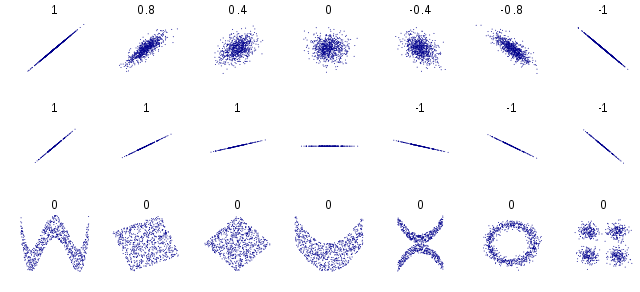
\includegraphics[width=0.9\textwidth]{c5.cor.01.png}
  \end{figure}
\end{frame}

\begin{frame}
  \frametitle{引言 | 相关 | 程度}
  \begin{table}
    \centering
    \rowcolors[]{1}{blue!20}{blue!10}
    \begin{tabular}{ccc}
      \hline
      \rowcolor{blue!50} 相关系数绝对值 & 相关程度 & 相关程度\\
      \hline
      约=1 & 完全相关 & Perfect correlated\\
      0.7~0.99 & 高度相关 & Highly correlated\\
      0.4~0.69 & 中度相关 & Moderately correlated\\
      0.1~0.39 & 低度相关 & Modestly correlated\\
      0.01~0.09 & 接近无相关 & Weakly correlated\\
      约=0 & 无相关 & ---\\
      \hline
    \end{tabular}
  \end{table}
  \begin{figure}
    \centering
    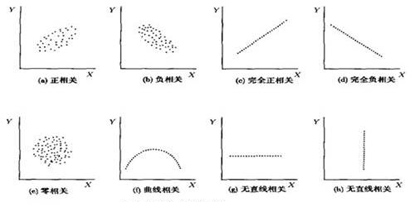
\includegraphics[width=0.7\textwidth]{c5.cor.02.jpg}
  \end{figure}
\end{frame}

\subsection{因果}
\begin{frame}
  \frametitle{引言 | 因果}
  \begin{block}{因果关系}
    因果关系是一个事件(即“因”)和第二个事件(即“果”)之间的关系,其中后一事件被认为是前一事件的结果。\\
    \vspace{0.5em}
一般来说,因果还可以指一系列因素(因)和一个现象(果)之间的关系。对某个结果产生影响的任何事件都是该结果的一个因素。直接因素是直接影响结果的因素,也即无需任何介入因素(介入因素有时又称中介因素)。从这个角度来讲,因果之间的关系也可以称为因果关联(causal nexus)。\\
    \vspace{0.5em}
原因和结果通常和变化或事件有关,还包括客体、过程、性质、变量、事实、状况;概括因果关系争议很多。对因果关系的哲学研究历史悠久,佛教和西方哲学家如亚里士多德在2000多年前就已经提出了因果,该问题仍是现代哲学的重要课题。
  \end{block}
\end{frame}

\begin{frame}
  \frametitle{引言 | 因果}
  \begin{figure}
    \centering
    
\includegraphics[width=0.8\textwidth]{c5.baoying.01.png}
  \end{figure}
\end{frame}

\subsection{相关 vs. 因果}
\begin{frame}
  \frametitle{引言 | 相关 vs. 因果}
  \begin{block}{相关 vs. 因果}
所谓事出必有因,按下遥控会转台,播种之后会发芽,阳光照耀天气暖,性行为导致生宝宝。人类能够看出两事之间的关联(动物有时也能),这种能力是很神奇的,因为这是生存的必要条件。但这种能力有时却错得离谱,让大家不分对错都能导出因果关系,即使是毫无关联的两件事也能够把它们兜在一起。我们只要看到一件事后面跟着另一件事发生,很容易就会以为前者是后者的原因,每当有相关数据或测量结果可以佐证时,更是如此。\\
    \vspace{0.5em}
    \alert{用相关性来证明因果关系,是现存最古老、也是最顽固的谬误。}
  \end{block}
\end{frame}

\begin{frame}
  \frametitle{引言 | 相关 vs. 因果}
  \begin{figure}
    \centering
    
\includegraphics[width=0.8\textwidth]{c5.vs.01.jpg}
  \end{figure}
\end{frame}

\begin{frame}
  \frametitle{引言 | 相关 vs. 因果}
  \begin{block}{你是如何混淆因果关系的?}
    \begin{itemize}
      \item “A越多,B越多”这样的相关性实际上有4种可能
        \begin{itemize}
          \item A导致B
          \item B导致A
          \item A和B同时被C导致
          \item A和B没有任何关系
        \end{itemize}
      \item 为什么我们总是错把“相关”当“因果”?因为我们本能——觉得相互靠近的东西一定是有关系的,同时出现的事件也一定是有关系的。
      \item 无数的错觉思维和错误归因不断发生
        \begin{itemize}
          \item 大众对新闻的错误归因。媒体为了提高点击率,经常使用这样的技巧:让新闻当事人的某个差异性特征出现在新闻上,从而让大众把“相关当因果”,觉得是这个差异性特征导致了他的行为。
          \item 盲目学习和模仿。我们经常盲目模仿成功者的特点,觉得模仿了他的特点,我们也能成功。(典型例子:成功人士与大学无用论。)
          \item 刻意规避和迷信。很多让你难以理解的祖传禁忌,实际上可能是当年某个相关事件的发生导致的。
        \end{itemize}
    \end{itemize}
  \end{block}
\end{frame}

\begin{frame}
  \frametitle{引言 | 相关 vs. 因果}
  \begin{figure}
    \centering
    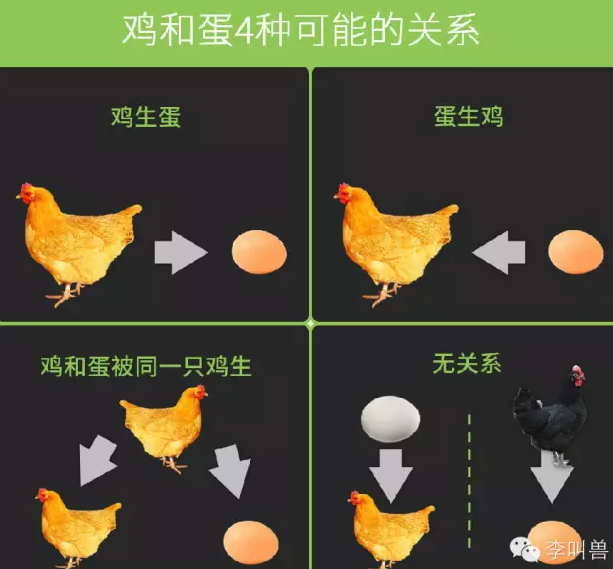
\includegraphics[width=0.4\textwidth]{c5.vs.05.jpg}
    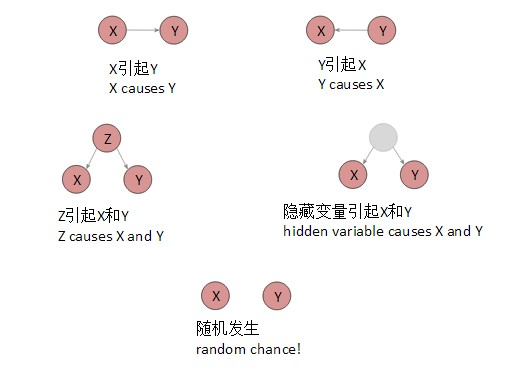
\includegraphics[width=0.5\textwidth]{c5.vs.06.jpg}
  \end{figure}
\end{frame}

\begin{frame}
  \frametitle{引言 | 相关 vs. 因果}
  \begin{figure}
    \centering
    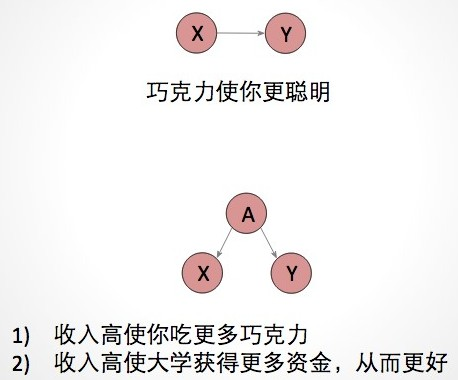
\includegraphics[width=0.4\textwidth]{c5.vs.07.jpg}
    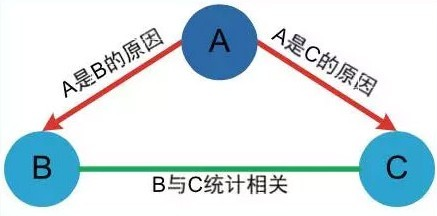
\includegraphics[width=0.5\textwidth]{c5.vs.08.jpg}
  \end{figure}
\end{frame}

\begin{frame}
  \frametitle{引言 | 相关 vs. 因果}
  \begin{figure}
    \centering
    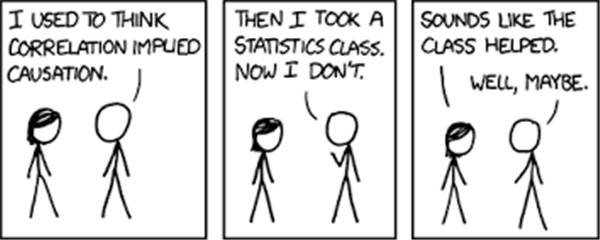
\includegraphics[width=0.8\textwidth]{c5.vs.02.jpg}\\
    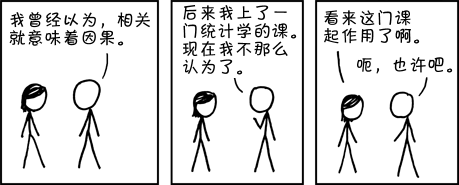
\includegraphics[width=0.8\textwidth]{c5.vs.03.png}
  \end{figure}
\end{frame}

\begin{frame}
  \frametitle{引言 | 相关 vs. 因果}
  \begin{figure}
    \centering
    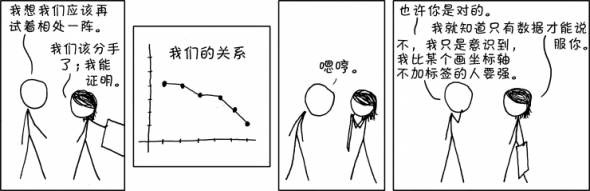
\includegraphics[width=0.9\textwidth]{c5.vs.04.jpg}
  \end{figure}
\end{frame}

\subsection{总结}
\begin{frame}
  \frametitle{引言 | 总结}
  \begin{block}{总结}
    \begin{itemize}
      \item \alert{两个事物之间的关联关系并不能用于说明其中一个将引起另一个的变化。}
      \item 所谓的“相关”往往是通过相关系数这个令人信服的精确数值来证明事物之间存在关联关系,它可以有多种不同的类型。
      \item 联合变动的一种普遍形式是存在着真实的关系,但却无法确定何为因何为果。有时因果可以不时地交换位置,或者实际上互为因果。
      \item 各种相关关系中,最富戏剧性的是虽然所有变量相互间没有任何影响,但是的确存在着显著的相关。
      \item 相关显示了一种趋势,而这种趋势通常并不是那种一对一的理想关系。
    \end{itemize}
  \end{block}
\end{frame}

\section{案例解析}
\subsection{引言}
\begin{frame}
  \frametitle{案例 | 引言}
  \begin{block}{引言}
两个事物之间的关联关系并不能用于说明其中一个将引起另一个的变化。但是我们却并不总是能够轻易地识别出,我们时不时错误地将关联关系判断为因果关系。特别是,当这种关系乍一看真像那么回事时,又或者它迎合了人们的惯常思维,这时你就更缺乏考究正误的动力了。\\
\vspace{0.5em}
由于存在偶然性,对于一些根本不可能发生的事情,你或许仍然能够收集数据证明其存在。但是如果你重新收集数据,或许第二组数据就无法证明这个结论了。\alert{任意两个事物或两组特性之间,在利用小样本后,都能建立显著地相关关系。}\\
\vspace{0.5em}
另一个需要留意的是,超过了推断相关关系的数据范围而得出的结论。正相关到了一定的程度后便急剧地转为负相关。\\
\vspace{0.5em}
某种相关关系也许是真实的,它依据的也是真实的因果关系,但同样也可能毫无意义,无法凭此做出行为决策。
  \end{block}
\end{frame}

\begin{frame}
  \frametitle{案例 | 引言}
  \begin{block}{物理学关系}
离灯越远,你就越看不清手中的书,也就是说,当距离增大时,光线的密度将减少。这些物理学的关系一般具有确定的相关。然而,来自商业、社会学或是医学的数据却很难如此清晰。
  \end{block}
  \vspace{-0.5em}
  \begin{figure}
    \centering
    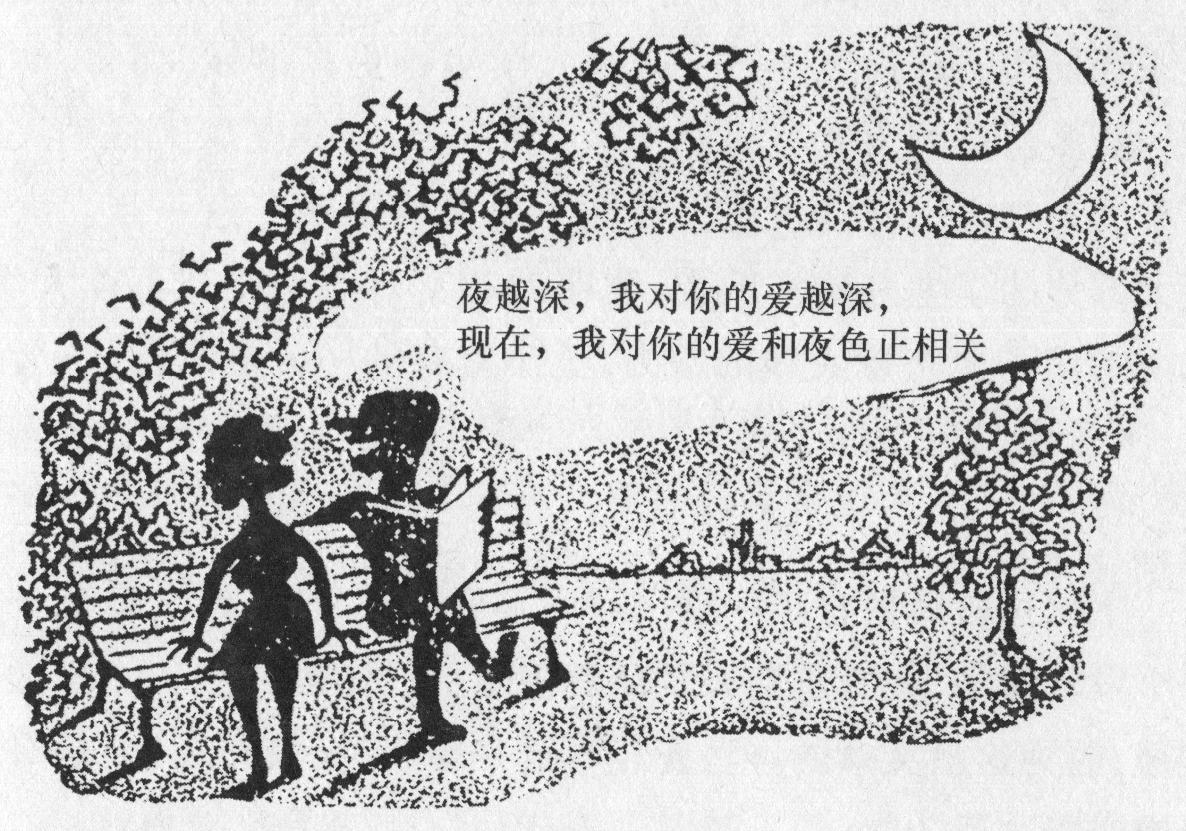
\includegraphics[width=0.7\textwidth]{c5.case.night.01.png}
  \end{figure}
\end{frame}

\subsection{精品案例}
\begin{frame}
  \frametitle{案例 | 抽烟 vs. 成绩}
  \begin{block}{现象}
    抽烟者的大学成绩比不抽烟者的差。
  \end{block}
  \pause
  \begin{block}{结论与推论}
    \begin{itemize}
      \item 在通往好成绩的道路上,需要忍受放弃抽烟带来的痛苦。
      \item 抽烟使人的头脑变笨。
    \end{itemize}
  \end{block}
  \pause
  \begin{block}{实验}
    整个研究过程是正确进行的:样本的容量足够大,而且经过了认真、仔细的挑选,相关关系的确十分显著,等等。
  \end{block}
\end{frame}

\begin{frame}
  \frametitle{案例 | 抽烟 vs. 成绩}
  \begin{block}{解析}
    更大的可能性:是两个因素并不互为因果,而同为第三个因素的产物。可能是那些不把读书当回事、爱社交的学生更偏爱抽烟?又或者是否可以从别的相关关系上找到线索?例如,性格与成绩之间的相关关系,它们之间的相关性比成绩与智力之间的还要高些。也许,性格外向的学生比性格内向的更爱抽烟。
  \end{block}
\end{frame}

\begin{frame}
  \frametitle{案例 | 牛奶 vs. 癌症}
  \begin{block}{警告}
    一篇医学文章曾严厉警告:喝牛奶的人群,他们癌症的发病率在上升。在英格兰、明尼苏达州、威斯康辛州、瑞士,这些牛奶产量和消费量极大的地区,癌症有上升趋势,而牛奶十分稀缺的锡兰却极少发生癌症病例。更进一步的证据是,在牛奶消费量少的美国南部地区癌症病例也相对较少。文章还指出,牛奶消费量极大的英国妇女患癌症的概率是很少喝牛奶的日本妇女的18倍。
  \end{block}
  \pause \pause \pause \pause
  \begin{block}{解析}
更深入地挖掘下去,会发现还有很多因素都可用于解释癌症发病率的提高,其中有一个因素就十分具有说服力,癌症主要发生在中年或者老年人身上。而发病率高的瑞士和前面提到的那些州,其居民寿命相对较长。研究期间英国妇女的平均寿命比日本妇女长12岁。
  \end{block}
\end{frame}

\begin{frame}
  \frametitle{案例 | 妇女年龄 vs. 脚尖角度}
  \begin{block}{研究}
    在研究年龄与妇女某些生理特征的关系时,测量了妇女走路时两脚分开的角度,你将发现年龄较长的妇女两脚分开的角度总是比较大。
  \end{block}
  \pause
  \begin{block}{结论}
    \begin{itemize}
      \item 脚尖朝外走路促使人变老。
      \item 年龄的增长造成脚尖角度的增大,而且大部分妇女随着年龄增长,脚尖的角度在不断增大。
    \end{itemize}
  \end{block}
  \pause \pause \pause \pause
  \begin{block}{解析}
任何此类的结论都可能是错误,而且无法得到证实。只有当对同样一些妇女或者基本上同等的群体进行一段时间的研究后,你才能得出合理的结论。因为这可以排除一些因素的影响,比如说,年纪大的女性在其年轻时期可能被告知应该脚尖向外走路,而年轻女性却在一个不鼓励脚尖朝外的年代学习走路。
  \end{block}
\end{frame}

\begin{frame}
  \frametitle{案例 | 跳蚤 vs. 健康}
  \begin{block}{信条}
    英国新赫布里底群岛土著居民的信条:身上的跳蚤会带来健康。
  \end{block}
  \begin{figure}
    \centering
    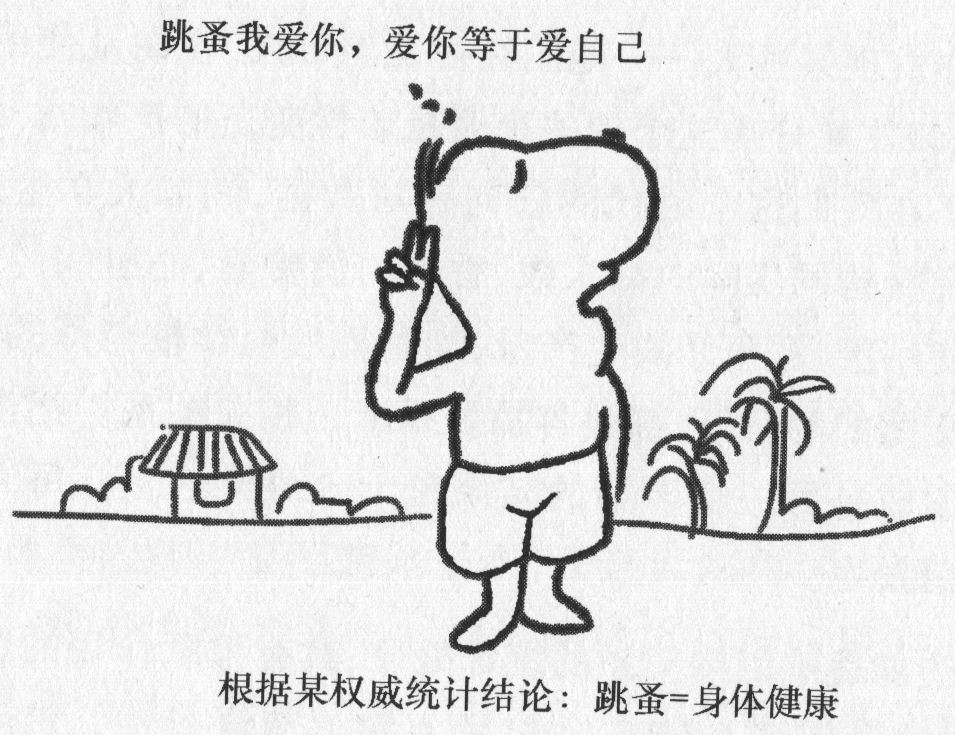
\includegraphics[width=0.7\textwidth]{c5.case.health.01.png}
  \end{figure}
\end{frame}

\begin{frame}
  \frametitle{案例 | 跳蚤 vs. 健康}
  \begin{block}{现象}
    通过几个世纪的观察,土著居民发现健康人的身上总有一些跳蚤,而身体羸弱的人身上通常没有跳蚤。
  \end{block}
  \pause
  \begin{block}{结论}
    跳蚤使人身体健康,每个人身上都应该有跳蚤。
  \end{block}
  \pause \pause \pause \pause
  \begin{block}{解析}
    \begin{itemize}
      \item 观察本身是正确的,因为它经历了多年来人们随意的检验,但这并不意味着这些土著居民的结论也是正确的。
      \item 更细心的观察者最终发现了新赫布里底群岛的真相:在大多数情况下,几乎每个居民身上都有跳蚤,这是正常情况。然而,当人们发烧(说不定还是跳蚤引起的)时,随着体温上升,跳蚤不能承受高温而引起的不适,因此就会离开。这里人们完全将因果关系扭曲、颠倒甚至混合了。
    \end{itemize}
  \end{block}
\end{frame}

\subsection{其他案例}
\begin{frame}
  \frametitle{案例 | 其他 | 海参 vs. 聪明}
  \begin{block}{实验}
在一定的人群中统计一下他们是否平时常吃海参,挑选出常吃海参的一组和不常吃海参的一组。然后进行智商测试,对总体结果进行统计,看看哪一组智商平均值更高,或者直接统计吃海参频率和智商之间的相关系数。
  \end{block}
  \pause
  \begin{block}{结论与推论}
    \begin{itemize}
      \item 如果常吃海参的一组平均智商得分更高,那么研究人员就会得出结论:常吃海参和智商高之间是呈正相关的关系的。
      \item 海参吃得越多智商就越高哦!为了提高智商赶紧吃海参吧!
    \end{itemize}
  \end{block}
\end{frame}

\begin{frame}
  \frametitle{案例 | 其他 | 海参 vs. 聪明}
  \begin{block}{解析}
海参和聪明之间的正相关性,有可能是因为经常吃到海参的家庭一般比较富裕,而富裕的家庭通常可以给孩子提供更好的教育资源,以使得孩子更聪明;也可能是有一个或者多个基因,同时起到了使人喜欢吃海参和提升智商两种作用。如果不排除这些其他可能性,说吃海参可以导致更聪明的说法就是不可信的。
  \end{block}
\end{frame}

\begin{frame}
  \frametitle{案例 | 其他 | 牧师 vs. 朗姆酒}
  \begin{block}{现象}
 在1860年到1940年间,美国东北部新英格兰地区卫理公会牧师数量呈现上升趋势,而其中最大的城市波士顿进口的古巴朗姆酒数量也随之增加,二者增加的趋势极其相似。
    \end{block}
  \pause
  \begin{block}{结论}
卫理公会牧师肯定在那段时间抢购了大量的朗姆酒。
  \end{block}
  \pause \pause \pause \pause
  \begin{block}{解析}
真正驱动二者数量上升的因素另有乾坤——人口增长。
  \end{block}
\end{frame}

\begin{frame}
  \frametitle{案例 | 其他 | 环球影城 vs. 汽车销量}
  \begin{figure}
    \centering
    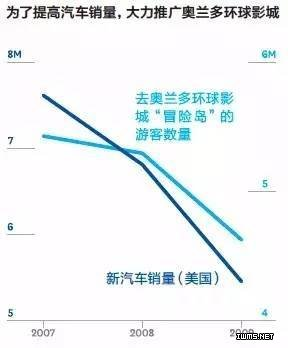
\includegraphics[width=0.5\textwidth]{c5.case.other.01.png}
  \end{figure}
\end{frame}

\begin{frame}
  \frametitle{案例 | 其他 | 失足淹死 vs. 失踪电影}
  \begin{figure}
    \centering
    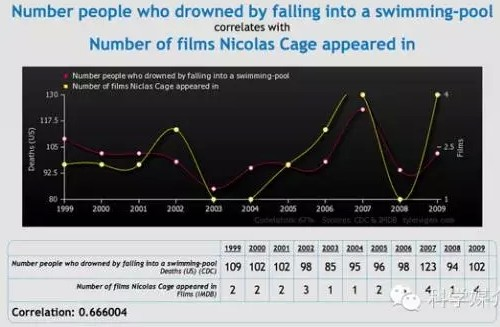
\includegraphics[width=0.9\textwidth]{c5.case.other.02.jpg}
    \caption{失足跌入游泳池淹死的人数与尼古拉斯凯奇出演的失踪电影数量呈正相关。}
  \end{figure}
\end{frame}

\begin{frame}
  \frametitle{案例 | 其他 | 蜜蜂 vs. 大麻}
  \begin{figure}
    \centering
    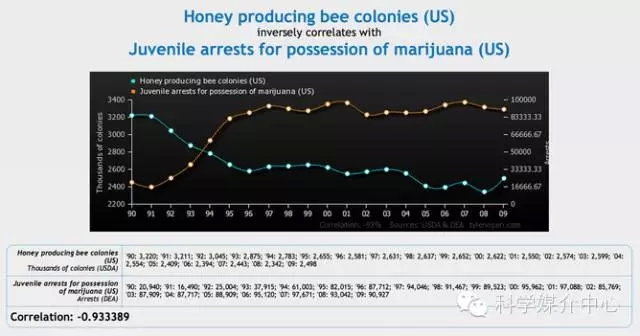
\includegraphics[width=0.9\textwidth]{c5.case.other.03.jpg}
    \caption{美国蜜蜂蜂群数量与因持有大麻被逮捕的美国青少年数量呈负相关。}
  \end{figure}
\end{frame}

% \begin{frame}
%   \frametitle{案例 | 其他 | 逻辑小测验}
%   \begin{block}{逻辑小测验}
%     \begin{itemize}
%       \item 气温正在升高,东非高原的疟疾病例愈来愈多,所以全球变暖正使得东非高原的疟疾病例数增多。
%       \item 气温正在升高,有种青蛙正逐渐灭绝,所以全球变暖正在让这种青蛙灭绝。
%       \item 气温正在升高,诺福克郡的海岸线正受到侵蚀,所以全球变暖正在侵蚀诺福克的海岸线。
%     \end{itemize}
%   \end{block}
% \end{frame}

\begin{frame}
  \frametitle{案例 | 其他}
  \begin{itemize}
    \item 游泳死亡人数越高,冰糕卖得越多,也就是游泳死亡人数和冰糕售出量之间呈正相关性,我们可以由此得出结论说吃冰糕就会增加游泳死亡风险吗?
    \item B学校学生毕业后拿到的平均工资更高,接受B学校的教育是导致工作较好的原因吗?
    \item 吸烟的人精神压力水平较大,那么吸烟会产生压力吗?
    \item 有孩子的人更加成熟,有孩子是成熟的原因吗?
    \item 海拔越高的地方我们感觉越冷。这是不是意味着海拔是导致温度低的原因?
    \item 震耳的音乐会引发青春痘?
    \item 体重过重的人活得比瘦子久,所以断定过胖可以延年益寿。
  \end{itemize}
\end{frame}

\begin{frame}
  \frametitle{案例 | 其他}
  \begin{itemize}
    % \item 在马萨诸塞州,长老教会会长的收入与哈瓦那朗姆酒的价格之间密切相关。
    \item 某人未婚婶婶的数字和其骨骼中钙含量(负的相关关系)
    \item 枯草热、花粉过敏等和小麦的价格(负的相关关系)
    \item 鞋的大小和笔迹的可识别性(正的相关关系)
    % \item 学校教育和收入(正的相关关系)
    \item 外国人比例和刑事犯罪(正的相关关系)
    \item 冰激凌销售量与犯罪率(正的相关系数)
    \item 已婚男子活的时间更长
    \item 张三和李四的手表的时间具有很强的相关性
    \item 股票行情和裙子长短流行的方式具有惊人的相似性
    \item 学生的SAT成绩和其家里的电视机数量呈正相关关系
    \item SAT考试分数与家庭的汽车数量之间存在高度的相关性
    \item 在过去20年里激增的中国人均收入和上升的美国儿童自闭症确诊率之间有一个正相关且具有显著统计学意义的关系
  \end{itemize}
\end{frame}

\section{图说天下}
\begin{frame}
  \frametitle{穷人的大脑更小}
  \begin{figure}
    \centering
    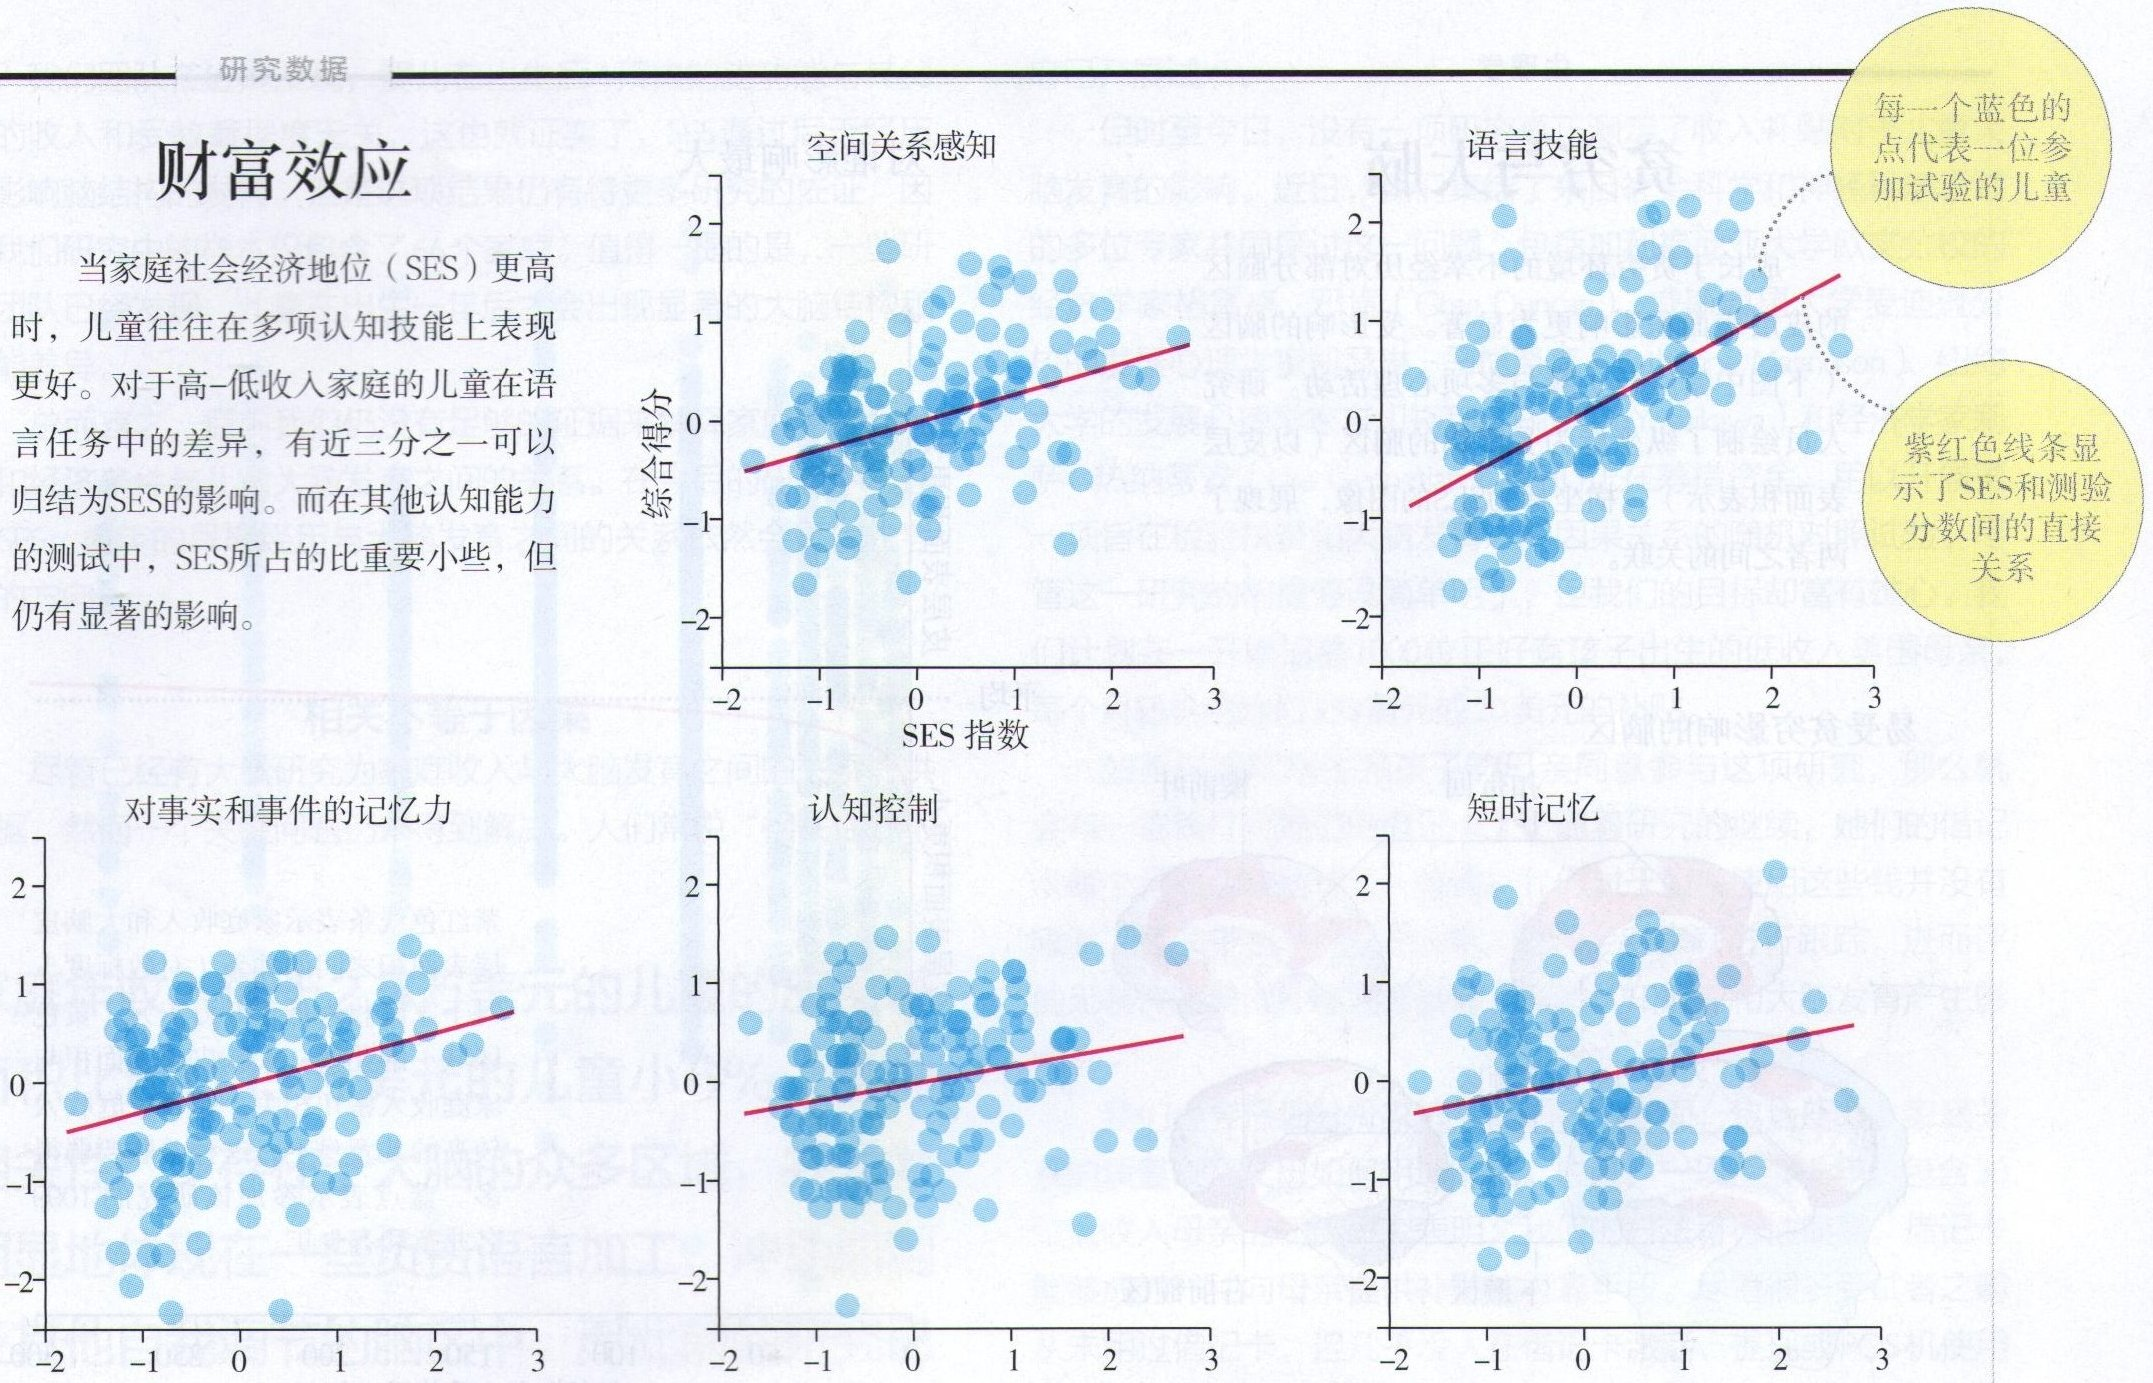
\includegraphics[width=0.9\textwidth]{c5.ses.01.jpg}
  \end{figure}
\end{frame}

\begin{frame}
  \frametitle{穷人的大脑更小}
  \begin{figure}
    \centering
    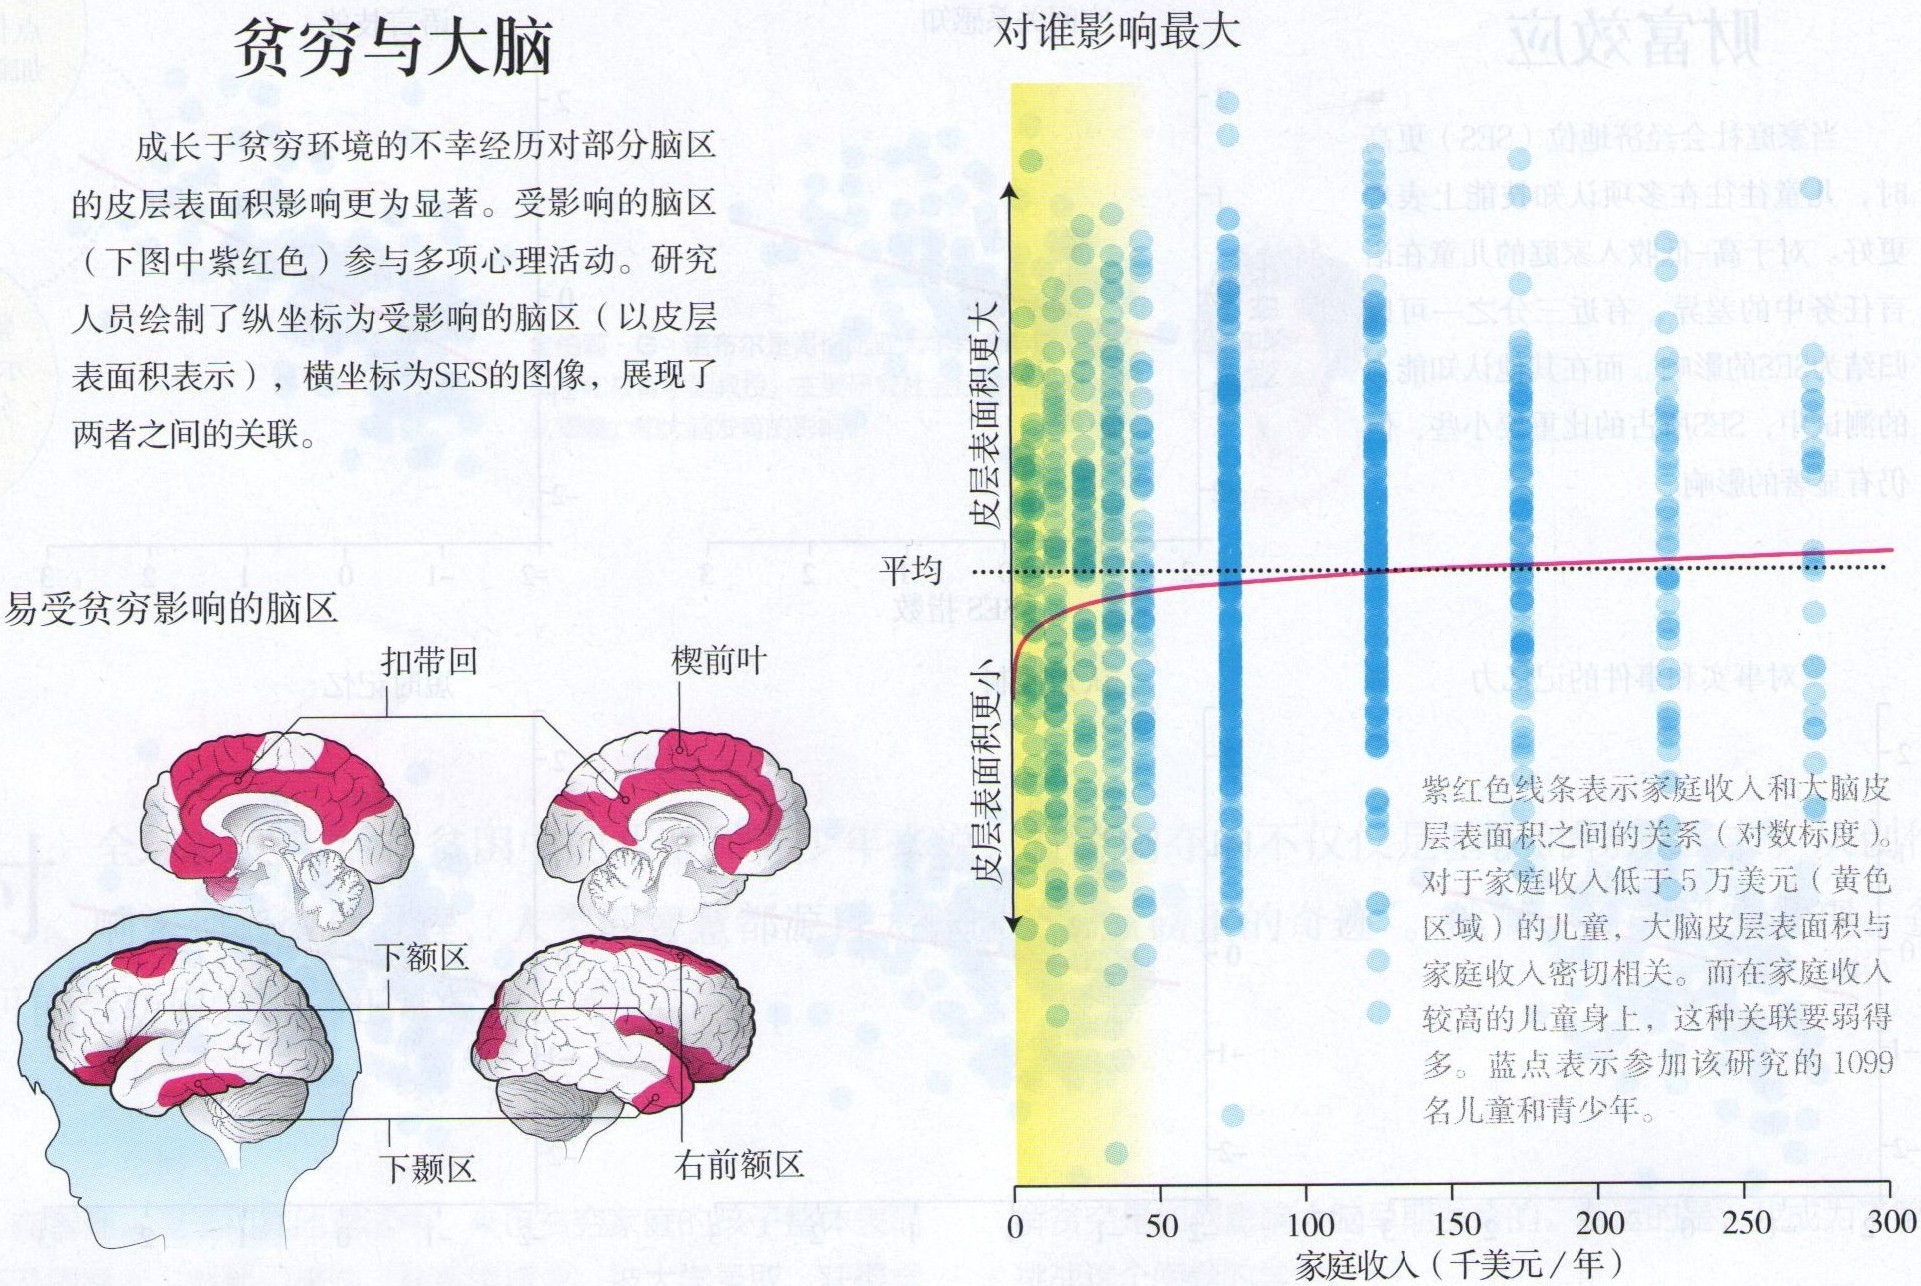
\includegraphics[width=0.9\textwidth]{c5.ses.02.jpg}
  \end{figure}
\end{frame}

\begin{frame}
  \frametitle{穷人的大脑更小}
  \begin{block}{随机对照试验}
为了研究因果关系,我们需要运用科学实验的黄金法则:随机对照试验。其中,随机分配的“治疗”组会接受某种干预,而同样随机分配的另一组则接受“对照”措施,这让我们能够判断这种干预对大脑发育的影响。
  \end{block}
  \begin{figure}
    \centering
    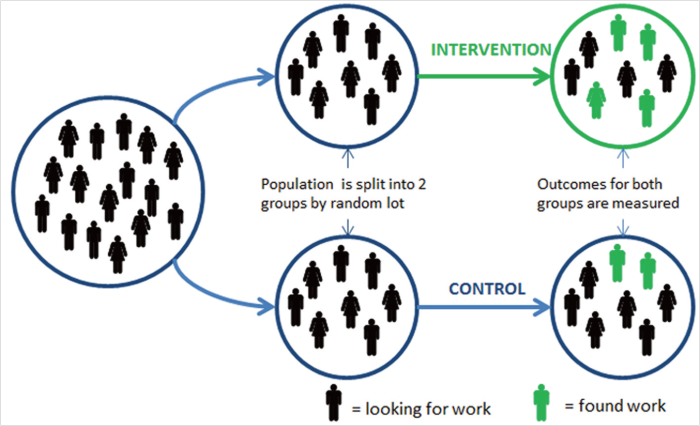
\includegraphics[width=0.7\textwidth]{c5.control.01.png}
  \end{figure}
\end{frame}

\begin{frame}
  \frametitle{运动悖论:锻炼无关减肥?}
  \begin{figure}
    \centering
    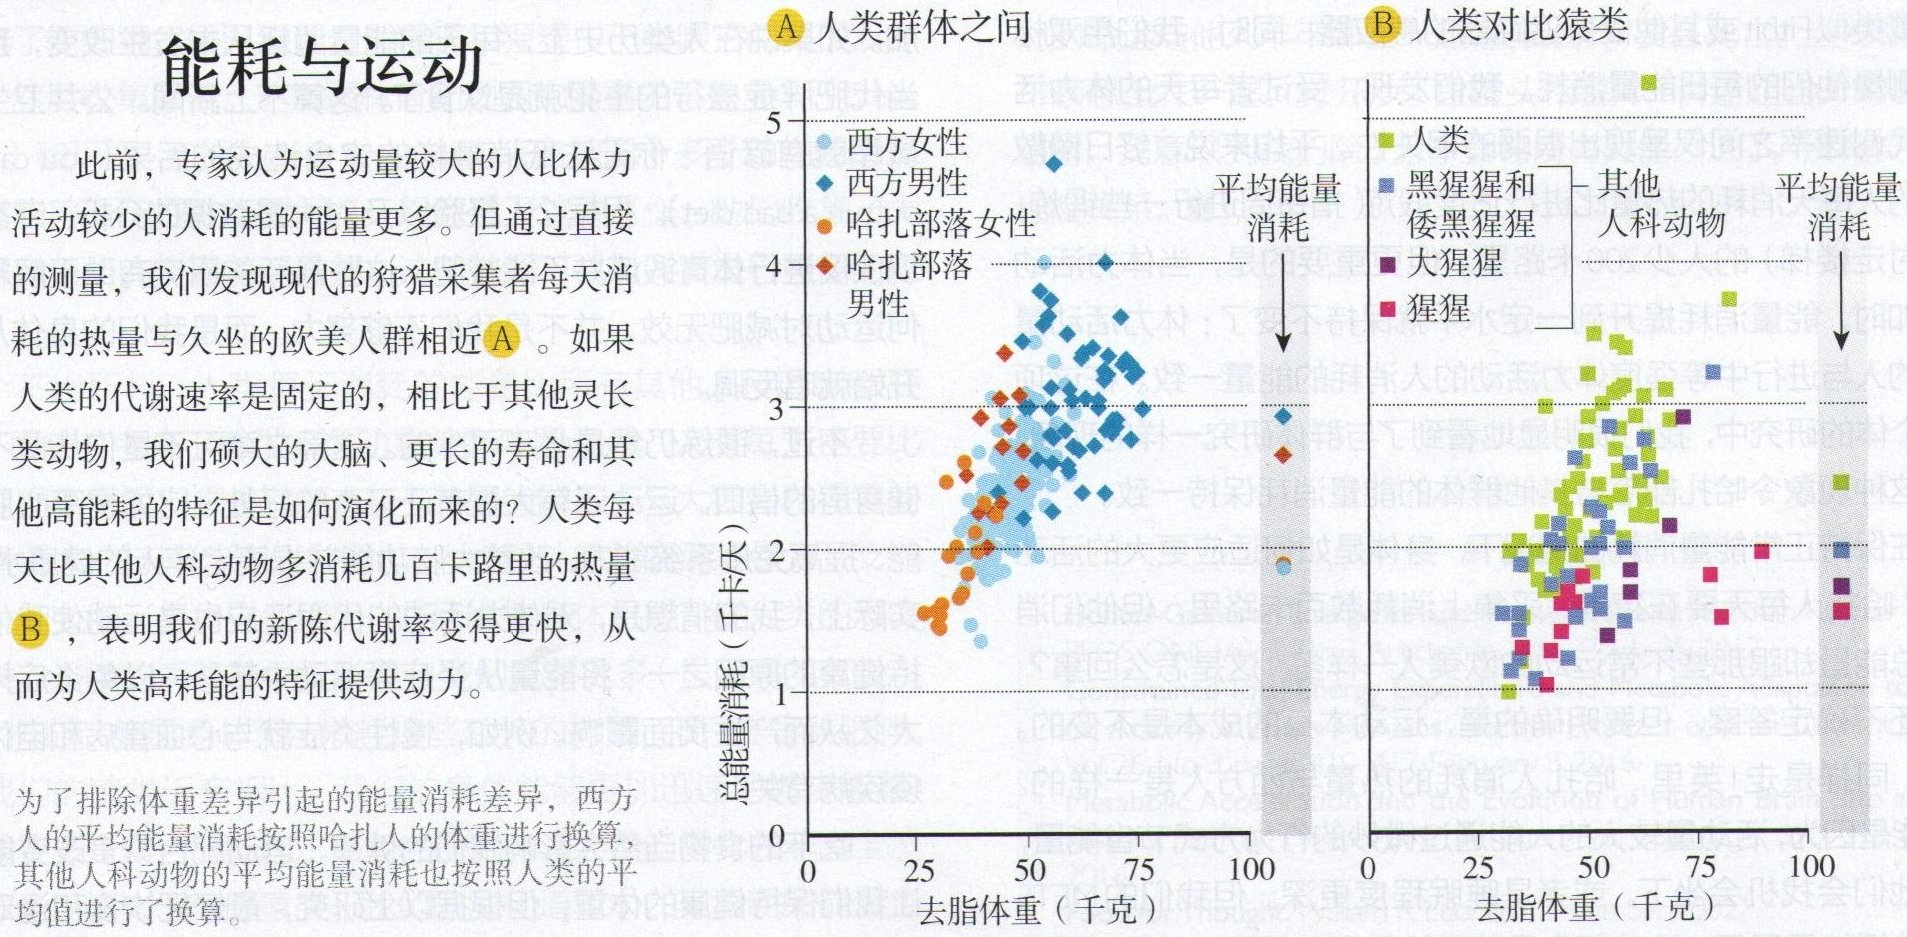
\includegraphics[width=\textwidth]{c5.sport.01.jpg}
  \end{figure}
\end{frame}




\section*{Acknowledgements}
\begin{frame}
  \frametitle{Powered by}
  \begin{center}
    
\includegraphics[width=9cm]{power.png}
  \end{center}
\end{frame}

\end{document}

